\documentclass[11pt]{article}
\usepackage{amsmath, amssymb, amscd, amsthm, amsfonts}
\usepackage{graphicx}
\usepackage{hyperref}
\usepackage{xcolor}

\usepackage[utf8]{inputenc}
\usepackage[a4paper, total={6in, 8in}]{geometry}
\usepackage{authblk}
\usepackage[T1]{fontenc}
\usepackage{mathtools}
\usepackage[thinc]{esdiff}
\usepackage{indentfirst}

\usepackage{listings}
\definecolor{codegreen}{rgb}{0,0.6,0}
\definecolor{codegray}{rgb}{0.5,0.5,0.5}
\definecolor{codepurple}{rgb}{0.58,0,0.82}
\definecolor{backcolour}{rgb}{0.95,0.95,0.92}
\lstdefinestyle{mystyle}{
    backgroundcolor=\color{backcolour},   
    commentstyle=\color{codegreen},
    keywordstyle=\color{magenta},
    numberstyle=\tiny\color{codegray},
    stringstyle=\color{codepurple},
    basicstyle=\ttfamily\footnotesize,
    breakatwhitespace=false,         
    breaklines=true,                 
    captionpos=b,                    
    keepspaces=true,                 
    numbers=left,                    
    numbersep=5pt,                  
    showspaces=false,                
    showstringspaces=false,
    showtabs=false,                  
    tabsize=2
}
\lstset{style=mystyle}

\oddsidemargin 0pt
\evensidemargin 0pt
\marginparwidth 40pt
\marginparsep 10pt
\topmargin -20pt
\headsep 10pt
\textheight 8.7in
\textwidth 6.65in
\linespread{1.2}

\newtheorem{theorem}{Theorem}
\newtheorem{lemma}[theorem]{Lemma}
\newtheorem{conjecture}[theorem]{Conjecture}

\newcommand{\rr}{\mathbb{R}}

\usepackage{color} %red, green, blue, yellow, cyan, magenta, black, white
\definecolor{mygreen}{RGB}{28,172,0} % color values Red, Green, Blue
\definecolor{mylilas}{RGB}{170,55,241}

\definecolor{mGreen}{rgb}{0,0.6,0}
\definecolor{mGray}{rgb}{0.5,0.5,0.5}
\definecolor{mPurple}{rgb}{0.58,0,0.82}
\definecolor{backgroundColour}{rgb}{0.95,0.95,0.92}

\lstdefinestyle{CStyle}{
    backgroundcolor=\color{backgroundColour},   
    commentstyle=\color{mGreen},
    keywordstyle=\color{magenta},
    numberstyle=\tiny\color{mGray},
    stringstyle=\color{mPurple},
    basicstyle=\footnotesize,
    breakatwhitespace=false,         
    breaklines=true,                 
    captionpos=b,                    
    keepspaces=true,                 
    numbers=left,                    
    numbersep=5pt,                  
    showspaces=false,                
    showstringspaces=false,
    showtabs=false,                  
    tabsize=2,
    language=C
}

\usepackage{titling}
\usepackage{braket}

\newcommand{\al}{\alpha}
\DeclareMathOperator{\conv}{conv}
\DeclareMathOperator{\aff}{aff}

\renewcommand{\thesubsection}{\thesection.\alph{subsection}} % 

\title{\textbf{N-Body Simulations of Spiral Galaxies}}
\author{Evan Shipley}
\affil{\textit{University of Maryland, Astronomy Department}}
\date{December 2022}

\begin{document}

\makeatletter
\renewcommand\section{\@startsection {section}{1}{\z@}%
                                   {-3.5ex \@plus -1ex \@minus -.2ex}%
                                   {2.3ex \@plus.2ex}%
                                   {\fontfamily{qpl}\Large\bfseries}}% from \Large
\renewcommand\subsection{\@startsection{subsection}{2}{\z@}%
                                     {-2.0ex\@plus -0.5ex \@minus -.1ex}%
                                     {1.0ex \@plus .1ex}%
                                 {\fontfamily{qpl}\large\bfseries}}% from \large
\renewcommand\subsubsection{\@startsection{subsubsection}{3}{\z@}%
                                     {-3.25ex\@plus -1ex \@minus -.2ex}%
                                     {1.5ex \@plus .2ex}%
                                     {\normalfont\large\bfseries}}% from \normalsize
\makeatother

\maketitle

\section{INTRODUCTION}
Astrophysical simulations give us an idea of what to look for in our observations of the universe based on the models used to generate them. In the study of galaxies in particular we can determine their location and age using redshifts and peculiar velocities (velocity wrt. a fixed point of reference.) We can compare their curvature or to theories of fluid dynamics and density waves. Along with this it is important to understand their mass distributions in any of their component parts such as a halo, disk, bulge, spiral arms and bar. In simulations we can see how the gravitational interactions between these structures as well as interactions with other nearby galaxies can induce the shapes we see naturally occurring in the universe. 

The idea that tidal interactions may be responsible for spiral arms was in fact first demonstrated by Holmberg (1941). In a now famous experiment, Holmberg modelled the interaction of two galaxies by representing the galaxies by a series of lightbulbs. The lightbulbs have initial velocities associated with them due to the initial velocities of each galaxy assumed for the interaction, and their rotation curves. A photocell is used to measure the total amount of light at any particular point in the galaxies. Since light obeys a inverse square law the same as gravity, the total light received by the photocell is equivalent to the total gravitational force at that point in the galaxy. This force, or rather acceleration, is then used to calculate how far to move the given lightbulb. This step is then repeated for all the lightbulbs used, and the whole process repeated for many steps. The results of this experiment showed clearly the development of tidal spiral arms.

In this project I design a simulation of a galaxy in the hope of it naturally evolving spiral arms. I start by generating masses representing stars randomly positioned in a doughnut shaped disk around a central black hole to represent stars for a given range of random stellar mass sizes. Predicting the motion of the stars at evolving time steps by incorporating Newton's Law of Universal Gravitation using galactic units of measurement.

\section{Why Simply Newton's Law?}
Only using Newton's Law to describe the forces between particles does actually complicate things more as this quote from Isaac Newton implies,

\begin{quote}
\textit{"The orbit of any one planet depends on the combined motion of all the planets, not to mention the actions of all these on each other. To consider simultaneously all these causes of motion and to define these motions by exact laws allowing of convenient calculation exceeds, unless I am mistaken, the forces of the entire human intellect."—Isaac Newton}
\end{quote}

Simulating dark matter fields or using the equations of motion per unit mass for a fluid would be a very interesting dive into complicated theories of forces. In the case of fluid dynamics, we could compare simulations of vortexes and mixtures of different densities to see spiral patterns emerge that resemble the what we see in galaxies. Solving equations like the Poisson and Navier-Stokes equation for this can be especially rigorous, but eventually proven analytically, and therefore has many applications so we see it already more than we might realize such as in image and shape processing. Fluid dynamics is definitely worth exploring more, but until then my simulation must suffice using gravity alone. As for the case of dark matter, I go into this deeper later on. However, my simulation does not incorporate it in its current form. 

In general relativity, the orbits for celestial bodies are geodesics of the space-time manifold that can be calculated using the curvature of this Minkowski Space. In the scale of galaxies, Newtonian physics approximates motions of celestial bodies reasonably well. Therefore, we could take the randomized scalar quantities of the value of the potential field to calculate a new trajectory for the celestial body based on its gravitational acceleration at each time step. Unfortunately, this simulation does not yet involve a scalar potential field to study the theory of dark matter. However, the key theory with or without dark matter is Newton's Law of Gravity.

\begin{align}
    \vec{F}&=m\vec{a}=m\ddot{\vec{r}}\\[1\baselineskip]
    \vec{F}_{Grav} &= -\frac{GM_1M_2}{r^2}\hat{r}=-\frac{GM_1M_2}{r^3}\vec{r}
\end{align}
where $M_1$ and $M_2$ are the masses of two objects, $r$ is the distance between them, and $G$ is Newton's gravitational constant.
Then, using $\vec{r}=x\hat{i}+y\hat{j}+z\hat{k}$ the vector equations above can be written as:
\begin{align}
    m(\ddot{x}\hat{i}+\ddot{y}\hat{j}+\ddot{z}\hat{j})=-\frac{GMm}{(x^2+y^2+z^2)^{3/2}}(x\hat{i}+y\hat{j}+z\hat{k})
\end{align}
If there are no outside forces/torques, Newton’s Laws for a gravitating system imply that total energy and total angular momentum are conserved and the system's center of mass is either stationary in the inertial frame, or moves with
constant velocity.


\section{Numerical Methods}
Given the equation governing the gradient of a function, Euler’s method sequentially calculates the value of the function, generating a series of values with the following
formula:
\begin{align}
f(x_{n+1})=f(x_n)+f'(x_n)dx
\end{align}
However, Euler's formula biases towards the starting end of the approximation and its approximations tend to gradually
diverge from the true values.
\begin{center}
\textbf{Euler approximation of $\frac{dx}{dt}=-x$}
\begin{flushright}
   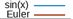
\includegraphics{legend} 
\end{flushright}
    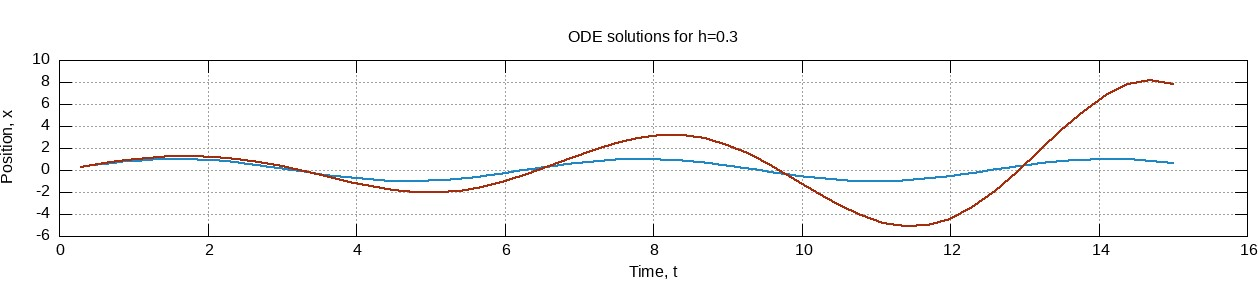
\includegraphics[width=1\textwidth]{Euler}
\end{center}
A better approximation, the fourth order Runge-Kutta method, was used instead. This method takes a weighted average of the gradient between two consecutive steps to estimate a balanced gradient that gives a better approximation at the end point.
In Runge-Kutta four the approximation at the end point is calculated using the weighted average of the slope at each of the four increments:
\begin{align}
&k_1=f(y(t_0),t_0)\\
&k_2=f(y(t_0)+k_1\frac{h}{2},t_0+\frac{h}{2})\\
&k_3=f(y(t_0)+k_2\frac{h}{2},t_0+\frac{h}{2})\\
&k_4=f(y(t_0)+k_3 h,t_0+h)\\
\end{align}
\begin{center}
    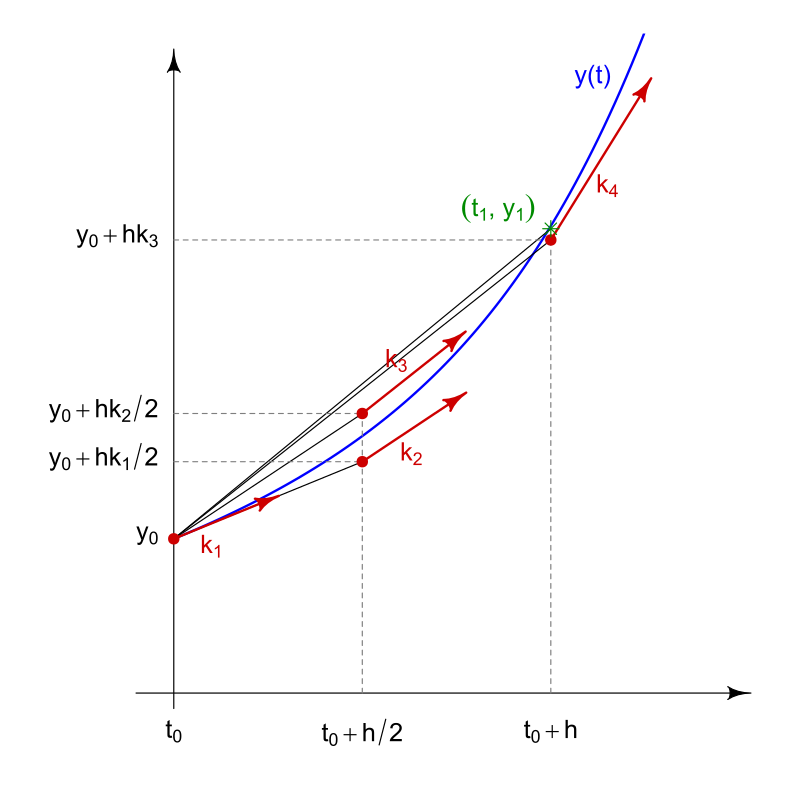
\includegraphics[width=0.5\textwidth]{slopes}
\end{center}
And their weighted average to estimate the end point:
\begin{align}
    y(t_0+h)=y(t_0)+\big(\frac{k_1}{6}+\frac{k_2}{3}+\frac{k_3}{3}+\frac{k_4}{6}\big)h
\end{align}
Now the numerical approximation of the solution of $\frac{dx}{dt}=-x$ is almost exactly the real solution $x=sin(t)$
\begin{center}
\textbf{Runge-Kutta approximation of $\frac{dx}{dt}=-x$}\\
    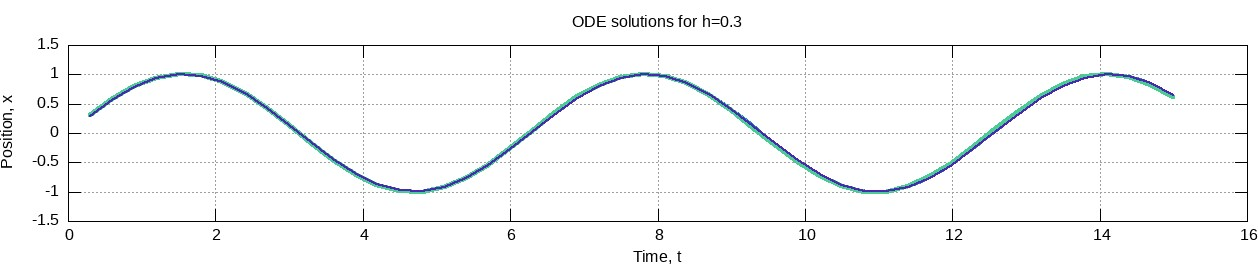
\includegraphics[width=1\textwidth]{RK4}
\end{center}
Accuracy of the orbital calculations are improved and the error rate is reduced. This comes at only a linear increase to the computation cost. Additionally, Runge-Kutta method is easily parallelized. Unfortunately, this simulation does not have the extremely advantageous processing speed benefit of parellization, yet.
\newpage
\section{Initial Parameters}

Many initial parameters for position and velocity are tested to check how the initial setup causes the system to behave. Simulations are tested with full disk shapes where there is no inner diameter and doughnut shapes with countless varying inner and outer diameters from tens and hundreds of parsecs to check the orbits on a scale the size of the Milky Way galaxies nucleus all the way out to inner and outer diameters as large as 10$^3$ and 1.7$\times 10^3$ parsecs respectively. In later trials I use some of the stars to generate a bulge by placing stars randomly inside a spherical volume one third the radius of the disk.

To generate point masses for the stars uniformly in the disk I used the following formula.
Let $u$ and $v$ be independent random numbers uniformly distributed in $[0,1)$, and let
$R_{\mathrm{in}}$ and $R_{\mathrm{out}}$ denote the inner and outer radii of the disk:
\begin{align}
    r   &= \sqrt{(R_{\mathrm{out}}^{2} - R_{\mathrm{in}}^{2})\,u + R_{\mathrm{in}}^{2}},\\
    \phi &= 2\pi v.
\end{align}
The Cartesian coordinates of each star are then
\begin{align}
    x = r\cos\phi,\qquad
    y = r\sin\phi,\qquad
    z = 0.
\end{align}

 Calculations for what a reasonable initial velocity for the stars would be are determined using various methods. For the disk the stars orbit in a counter-clockwise direction. If the stars were not in a doughnut shape with a significantly large inner radius on the order of 10$^3$ parsecs then the speeds required to keep the stars bound to reasonable orbit for a significant time period was their escape speed. This prevented them from falling in toward the center too quickly and being ejected out. These speeds are not in-line with the speeds we observe in the Milky Way.
 \begin{center}
\end{center}

\section{Mass Density and Long Lived Spirals}
Mass distributions are obtained by two ways: one is to use photometric data such as luminosity profiles assuming the mass-to-luminosity ratio, and the other is to apply dynamics to kinematical data based on the Virial theorem. Much work has been done using light to study mass distributions since was first done in the early 20th century by measuring stellar density in the solar neighborhood and multiplying by the volume of the Galaxy to get an estimate for the total number of solar mass stars in our Galaxy. This gave an approximate mass on the order of 10$^{11}\ M_\odot$. When it comes to dark matter and invisible masses like black holes, it is necessary to apply the dynamical method using kinematical data. The dynamical mass is calculated based on the Virial theorem which states that the kinetic and gravitational energies are in equilibrium for a dynamically relaxed system. For a rotating object such as the galactic disk, the balance between the gravitational and centrifugal forces is applied.

In simulations one should incorporate different stellar mass densities or dark matter densities in order to visualize how matter would interact under certain restrictions and compare it to observation. To begin several initial conditions need to be chosen: What kind of angular momentum will the baryonic matter in the system have? Will the model incorporate dark matter and will there be dark matter-baryon interactions (DMb)? In which case one might look at momentum transfer or thermal evolution. This could lead to predictions of galaxy spirals forming from differential rotation, dispersion relations, or swing amplification such as in fluid dynamics which in turn may produce density waves. Density waves could arise from other factors such as harmonic oscillations in the gravitational potential. 

One way to incorporate density waves leading to the formation of spiral arms is by modifying the density field. Fourier components of the density field that are used in the power spectrum are orthonormal within a cube. Thus, an approach to quantifying the galaxy density field is by using spherical harmonics. Spherical harmonics are an orthonormal set of functions on a sphere. They offer a natural way to smooth the data. 

In Bray’s 2010 paper, spherical harmonics were used to get the general solution for the density function. It is unrealistic to include all the spherical harmonic terms in a simulation. Only the real wave functions can guarantee the density function to be positive. The wave function given by Bray is of the form:
\begin{align}
   f = A_0 cos(\omega_0t)f_{\omega0,0}(r) + A_2 cos(\omega_2t − 2\phi) sin^2(\theta)r^2f_{ω2,2}(r) 
\end{align}
In a more detailed case where the effects of relativity are a concern we could study the potential well coming from a galaxy. This is unnecessary if we are only interested in the scale and shape of the galaxy and can just use Newtonian equations. After the wave function, f, is solved, the density function for dark matter, $\mu$DM, can be solved. From this the gravitational potential for dark matter can be solved. Finally, the gradient of this potential is taken to use as a force field to run the simulations.

\newline
I highly recommend the paper by Hubert L. Bray. Which has great introductions to general relativity and beautiful lifelike spiral galaxy simulations. There is a link in the Open Problems section of the paper meant to download the MATLAB simulations, but this link is broken. His code can be found on this updated link to his website \url{https://services.math.duke.edu/~bray/darkmatter/darkmatter.html}

\section{References}
\begin{tabbing}
Disk-Galaxy Density Distribution from Orbital Speeds using Newton's Law, K. Nicholson, 2018\\[0\baselineskip]
\ \ \ \ https://arxiv.org/abs/1801.05986\\[0\baselineskip]
The Mass Distribution and Rotation Curve in the Galaxy, Y. Sofue, 2013\\[0\baselineskip]
\ \ \ \ https://arxiv.org/abs/1307.8215\\[0\baselineskip]
Simulations of Spiral Galaxies, B. Hubert, B. Hamm. Y. Bei, Y. Guan, Z. Liu, 2017\\[0\baselineskip]
\ \ \ \ https://services.math.duke.edu/DOmath/DOmath2017/bei-guan-liu.pdf\\[0\baselineskip]
On Dark Matter, Spiral Galaxies, and the Axioms of General Relativiy, H. L. Bray, 2010\\[0\baselineskip]
\ \ \ \ https://arxiv.org/pdf/1004.4016\\[0\baselineskip]
Spiral Structures in Disk Galaxies, C. Dobbs, J. Baba 2014\\[0\baselineskip]
\ \ \ \ https://ned.ipac.caltech.edu/level5/March15/Dobbs/Dobbs\_contents.html\\[0\baselineskip]
The Density and Peculiar Velocity Fields of Nearby Galaxies, M. Strauss, J. Willick, 1995\\[0\baselineskip]
\ \ \ \ https://arxiv.org/pdf/astro-ph/9502079\\[0\baselineskip]
Review of the Universe, Fluid Dynamics and the Navier Stokes, universe-review.ca\\[0\baselineskip]
Modelling mass distribution of the Milky Way galaxy using Gaia’s billion-star map, Enbang Li, 2016\\[0\baselineskip]
\ \ \ \  https://arxiv.org/ftp/arxiv/papers/1612/1612.07781\\[0\baselineskip]
Cosmological Constraints on Dark Matter Interactions with Ordinary Matter, M. Buen-Abad, R. Essig, D, McKeen, Y. Zhong 2022\\[0\baselineskip]
\ \ \ \  https://arxiv.org/pdf/2107.12377
\end{tabbing}


\end{document}
